\documentclass[12pt,letterpaper,oneside]{article}
\renewcommand*{\title}{Intro to tensors}
\renewcommand*{\author}{Sam Grayson}

\usepackage[utf8]{inputenc}
\usepackage[T1]{fontenc}
\usepackage{lmodern}
\usepackage[english]{babel}
\usepackage[letterpaper, margin=1in]{geometry}
\usepackage{fancyhdr}
\usepackage{lastpage}
\usepackage{etoolbox}
\usepackage[pdftex,
	pdfauthor={\author},
	pdftitle={\title},
]{hyperref}
\usepackage{setspace}
\usepackage{mathtools} % imports amsmath
\usepackage{amssymb}
\usepackage[pdftex]{graphicx} % for \IncludeGraphics[width=1.0in]{picture.png}
\usepackage[usenames,dvipsnames,svgnames,table]{xcolor} % for \textcolor{gray}{hello world}
\usepackage{tikz} % for computer generated graphics

%%% fancy Header
\pagestyle{fancy}
\setlength{\headheight}{8.2pt}
\fancyhf{}
\lhead{\textcolor{gray}{{\title} {by \author}}}
\rhead{\textcolor{gray}{\thepage~of~\pageref{LastPage}}}
\makeatletter
\patchcmd{\headrule}{\hrule}{\color{gray}\hrule}{}{}
\makeatother

\DeclarePairedDelimiter{\norm}{\lVert}{\rVert}
%\DeclareListParser{\docsvlist}{,}
\newcommand{\vecl}[1]{
\renewcommand*{\do}[1]{##1 \\}
\begin{pmatrix}
  \docsvlist{#1}
\end{pmatrix}
}
\newcommand*{\vertbar}{\rule[-1ex]{0.5pt}{2.5ex}}

\begin{document}
\thispagestyle{empty}

\begin{center}
\textbf{\Large \title \\} \vspace{0.1cm}
\textit{\small by \author \\} \vspace{-1cm}
\end{center}

\onehalfspacing\ 

\section{Notes}

This tutorial is best understood if the reader has a basic familarity with linear algebra. This tutorial is designed to teach tensors as they are used in physics (as opposed to analytic geometry). As such, I will assume that vector spaces are finite-dimensional unless stated otherwise.

For further reading, consult:

\begin{itemize}
\item \url{https://en.wikipedia.org/wiki/Tensor}
\item \url{https://www.grc.nasa.gov/www/k-12/Numbers/Math/documents/Tensors_TM2002211716.pdf}
\item \url{http://www.learndev.org/dl/Science/TensorTechniquesInPhysics.pdf}
\item \url{http://www.springer.com/us/book/9783319127866}
\end{itemize}

\section{Review from linear algebra}

\subsection{Change of Basis}

When I say $$\vec{u} = \vecl{5, 3, 0},$$ I really mean $\vec{u} = 5 \hat{x} + 3 \hat{y} + 0 \hat{z}$ where $$\hat{x} = \vecl{1,0,0}\!, \hat{y} = \vecl{0,1,0}\!, \hat{z} = \vecl{0,0,1}$$. We generally the notation $\vec{e}_1}, \vec{e}_2}, \vec{e}_3}$ instead of $\hat{i}, \hat{j}, \hat{k}$ instead because it generalizes to $\mathbb{R}^n$. The components (also called coordinates) of $\vec{u}$ become the coefficients of $\vec{e}_i}$.

These are called the `standard' basis vectors. However any set of $n$ linearly-independent vectors can form a basis for an $n$-dimensional space. Suppose I call this the $d$-basis $$\left[  \vecl{1, 1, 0}\!, \vecl{1,-1,0}\!, \vecl{0,0,2}\!, \right].$$

$\vec{u}$ can be written as a linear combination\footnote{A linear combination of a bunch of vectors is the sum of products of scalars and vectors.} of $d$-vectors.\footnote{This can be verified by the reader from basic vector arithmetic.} $$\vec{u} = 4\vec{d}_1} + 1\vec{d}_2} + 0\vec{d}_3}.$$

Note that it has the same form of the expression $\vec{u} = 5 \vec{e}_1 + 3 \vec{e}_2 + 0 \vec{e}_3$. It is then natural to say that the coordinates of $\vec{u}$ are 4, 1, and 0 with respect to the basis $d$.

In some sonse $d$ is the `weird' basis and $e$ is the `standard' basis, but that choice is arbitrary. In this case, $d$ is just $e$ rotated by $45^\circ$ in the $xy$-plane and stretched out. There is no reason to prefer $e$. If we pretended that $d$ was the `standard basis', then $e$ would be $$\left[ \vecl{\frac 1 2, \frac 1 2, 0}, \vecl{\frac 1 2, -\frac 1 2, 0}, \vecl{0, 0, \frac 1 2} \right],$$ (because $\vec{e}_1} = \frac 1 2 \vec{d}_1} + \frac 1 2 \vec{d}_2} + 0 \vec{d}_3}$ which I put in the first column, likewise for $\vec{e}_2}$ in the second column, and $\vec{e}_3}$ in the third) and from that point of view, $e$ is the `weird basis'.

This can be expressed in the language of matrices

$$\vec{u} = 4\vec{d}_1} + 1\vec{d}_2} + 0\vec{d}_3} = \vecl{\vertbar & \vertbar & \vertbar \\ \vec{d}_1} & \vec{d}_2} & \vec{d}_3} \\ \vertbar & \vertbar & \vertbar \\}\vecl{4, 1, 0}\!.$$

In order to convert $d$-coordinates into standard coordinates, we just have to multiply by a matrix whose $i$th column is $\vec{d}_i}$. (I will write a subscript parenthesized $d$ to denote `coordinates with respect to $d$'). If you have a basis $d$, let $D$ be the matrix whose columns are vectors of $d$, and $\vec{u}_{(d)}$ be the coordinates with respect to that basis $d$, 

$$\vec{u} = D \vec{u}_{(d).}$$

This gives us a method to solve for the $d$-coordinates. It can be challenging to decompose a vector $\vec{v}$ into a linear combination of $\vec{d}_1}, \vec{d}_2}, \vec{d}_3}$. But by manipulating the previous equation,

$$D^{-1} \vec{u} = \vec{u}_d$$

We know $D$ is invertible because its columns are vectors of a basis, which means they are linearly independent, which means the rank is the dimension, which means it is invertble.

\subsubsection{Sources}

\href{https://en.wikipedia.org/wiki/Change_of_basis}{Wikipedia: Change of Basis}

\subsection{Application: diagonalizing matrices for fun and profit}

This has some neat consequences that you might remember from linear algebra. If not, read on!

Some problems are easier to solve in another basis. Like multiplying an $n \times n$ matrix, $B$, by a vector, $\vec{x}$. If $B$ has $n$ linearly independent eigenvectors $\vec{u_i}$ \footnote{Recall that an eigenvector, $\vec{u_i}$, is a vector where multiplying by $B$ does the same thing as multiplying by a scalar, $\lambda_i$ ($B\vec{u_i} = \lambda_i \vec{u_i}$). As you can imagine, most vectors are not eigenvectors. Most matrices don't have any. But on the off-chance that the matrix has $n$ linear independent eigenvectors\dots} and $\vec{x}$ were expressed in coordinates relative to the eigenvectors of $B$, $\vec{x} = c_1 \vec{u_1} + \dotsb + c_n \vec{u_n}$, then $$B\vec{x} = B(c_1 \vec{u_1} + \dotsb + c_n \vec{u_n}) = c_1 B \vec{u_1} + \dotsb + c_n B \vec{u_n} = c_1 \lambda_1 \vec{u_1} + \dotsb + c_n \lambda_n \vec{u_n},$$so each coordinate (coordinate relative to basis $u$) would just get multiplied by its eigenvalue, $\lambda_i$, and you would have the coordinates of the result (relative to basis $u$).

If $\vec{x}_{(u)} = \vecl{c_1, \vdots, c_n}$ and $\Lambda = \begin{pmatrix}
  \lambda_1 & 0 & 0 \\
  0 & \ddots & 0 \\
  0 & 0 & \lambda_n \\
\end{pmatrix}$, then\footnote{remember $[\vec{b}]_{(u)}$ means the coordinates of $\vec{b}$ relative to basis $u$.} $[B\vec{x}]_{(u)} = \Lambda\vec{x}_{(u)}$, because $\Lambda$ just multiplies the $i$th coordinate by $\lambda_i$.

Now to convert the result from $u$ coordinates into standard coordinates, we just have to multiply by $U$ where $U$ is a matrix whose columns are vectors of the basis $u$ (which were also eigenvectors). And to put $\vec{x}$ into $u$ coordinates, I have to mulitply by $U^{-1}$

\begin{enumerate}
\item Write $\vec{x}$ in $u$-coordinates: $U^{-1}\vec{x}$
\item Multiply the $i$th coordinate \textbf{relative to the eigenvectors} by $\lambda_i$: $\Lambda U^{-1} \vec{x}$
\item Convert from $u$-coordinates to standard coordinates: $U\Lambda U^{-1} \vec{x}$
\item And that does the same thing as $B\vec{x}$: $B\vec{x} = U\Lambda U^{-1} \vec{x}$
\end{enumerate}

Since linear transformations are unique (if $B\vec{x} = C\vec{x}$ for all $\vec{x}$, then $B = C$). Finally we arrive at $B = U \Lambda U^{-1}$, which is called the Spectral Decomposition of $B$. $\Lambda$ is called a diagonal matrix because everything off of the diagonal is zero. $B$ is called `diagonalized'.

Lets say you wanted to compute $B^i$. This is usually required for simulating dynamical systems where $B$ times the current vector is the next vector. However it quickly gets difficult to compute even for small $i$ if $B$ is highly-dimensional (if it were, say, a 10 by 10 matrix). For my next magic trick, I will make the computational complexity of this problem dissappear!

Suppose you complete the method I described above and find a $\Lambda$ and $U$ such that $B = U \Lambda U^{-1}$. Then $$B^{3} = B B B = (U \Lambda U^{-1}) (U \Lambda U^{-1})  (U \Lambda U^{-1}) = U \Lambda (U^{-1}U) \Lambda (U^{-1} U) \Lambda U^{-1} = U \Lambda^3 U^{-1},$$
but $\Lambda$ is a diagonal matrix, so you only have to take $n$ scalars to the third power\footnote{This generalizes to the $i$th power $B^i = U \Lambda^i U^{-1}$, where $\Lambda^i$ is a diagonal matrix.},
$$\Lambda^3 = \begin{pmatrix}
\lambda_1^3 & 0 & 0 \\
  0 & \ddots & 0 \\
  0 & 0 & \lambda_n^3 \\
\end{pmatrix}$$

If you have heard of Markov Processes, then you might remember that their steady-state solutions (basically $B^\infty$) are the eigenvectors whose eigenvalues are non-zero of the transition matrix. If you were to compute $B^\infty$ with this method, then $$\lambda_i^\infty = \begin{cases}
  \infty & \lambda_i > 1~~ \text{(good thing that never happens in a Markov process)} \\
  1 & \lambda_i = 1 \\
  0 &  0 \leq \lambda_i < 1 \\
  \mathrm{D.N.E} & \lambda < 0 ~~\text{(good thing that never happens in a Markov process)} \\
\end{cases}
$$

\subsection{Application: Fourier transform}

Some problems are easier to solve in another basis. Like cranking up the bass on your ear-pounding subwoofer for the person next to you at a red light as they begin to roll down the window (make a system that will amplify all of the low notes in an audio stream). But you aren't just any annoying person; You are an annoying person who understands physics and math, and you want to if not build, at least describe this system yourself. Who needs engineers!

Vector spaces are useful for more than just spatial geometry. You can make a vector space on the set of `well-behaved\footnote{By `well-behaved' I mean `Lebesgue-integrable'}' functions. A vector space can be composed of anything that you can multiply-by-a-scalar or add-together. Scalar multiplication works $a \vec{f}$ is like $a f(x)$, and $\vec{f} + \vec{g} = f(x) + g(x)$, where $x$ remains a free parameter.

$\vec{f}_\xi(x) = \exp(-2 \pi i \xi x)$ where $\xi \in \mathbb{R}$ form an (infinite) basis for this space. That's pretty weird and pretty important. But just like any vector in good-ol' three-dimensional space can be written as $c_1 \vec{e}_1 + c_2 \vec{e}_2 + c_3 \vec{e}_3 = \sum_{i=1}^3 c_i \vec{e_i}$, every well-behaved function, $g(x)$, can be written as $g(x) = \sum_{\xi \in \mathbb{R}} c_\xi \vec{f_\xi}(x) = c_\xi \exp(-2 \pi i \xi x)$. The Fourier transform computes the coordinates $c_\xi$ (the coordinate $c_\xi$ is called the amplitude of the frequency $\xi$). \textit{The Fourier Transform is just a way of changing basis to the $\exp(-2 \pi i \xi x)$ basis!}

\begin{figure}
\begin{center}
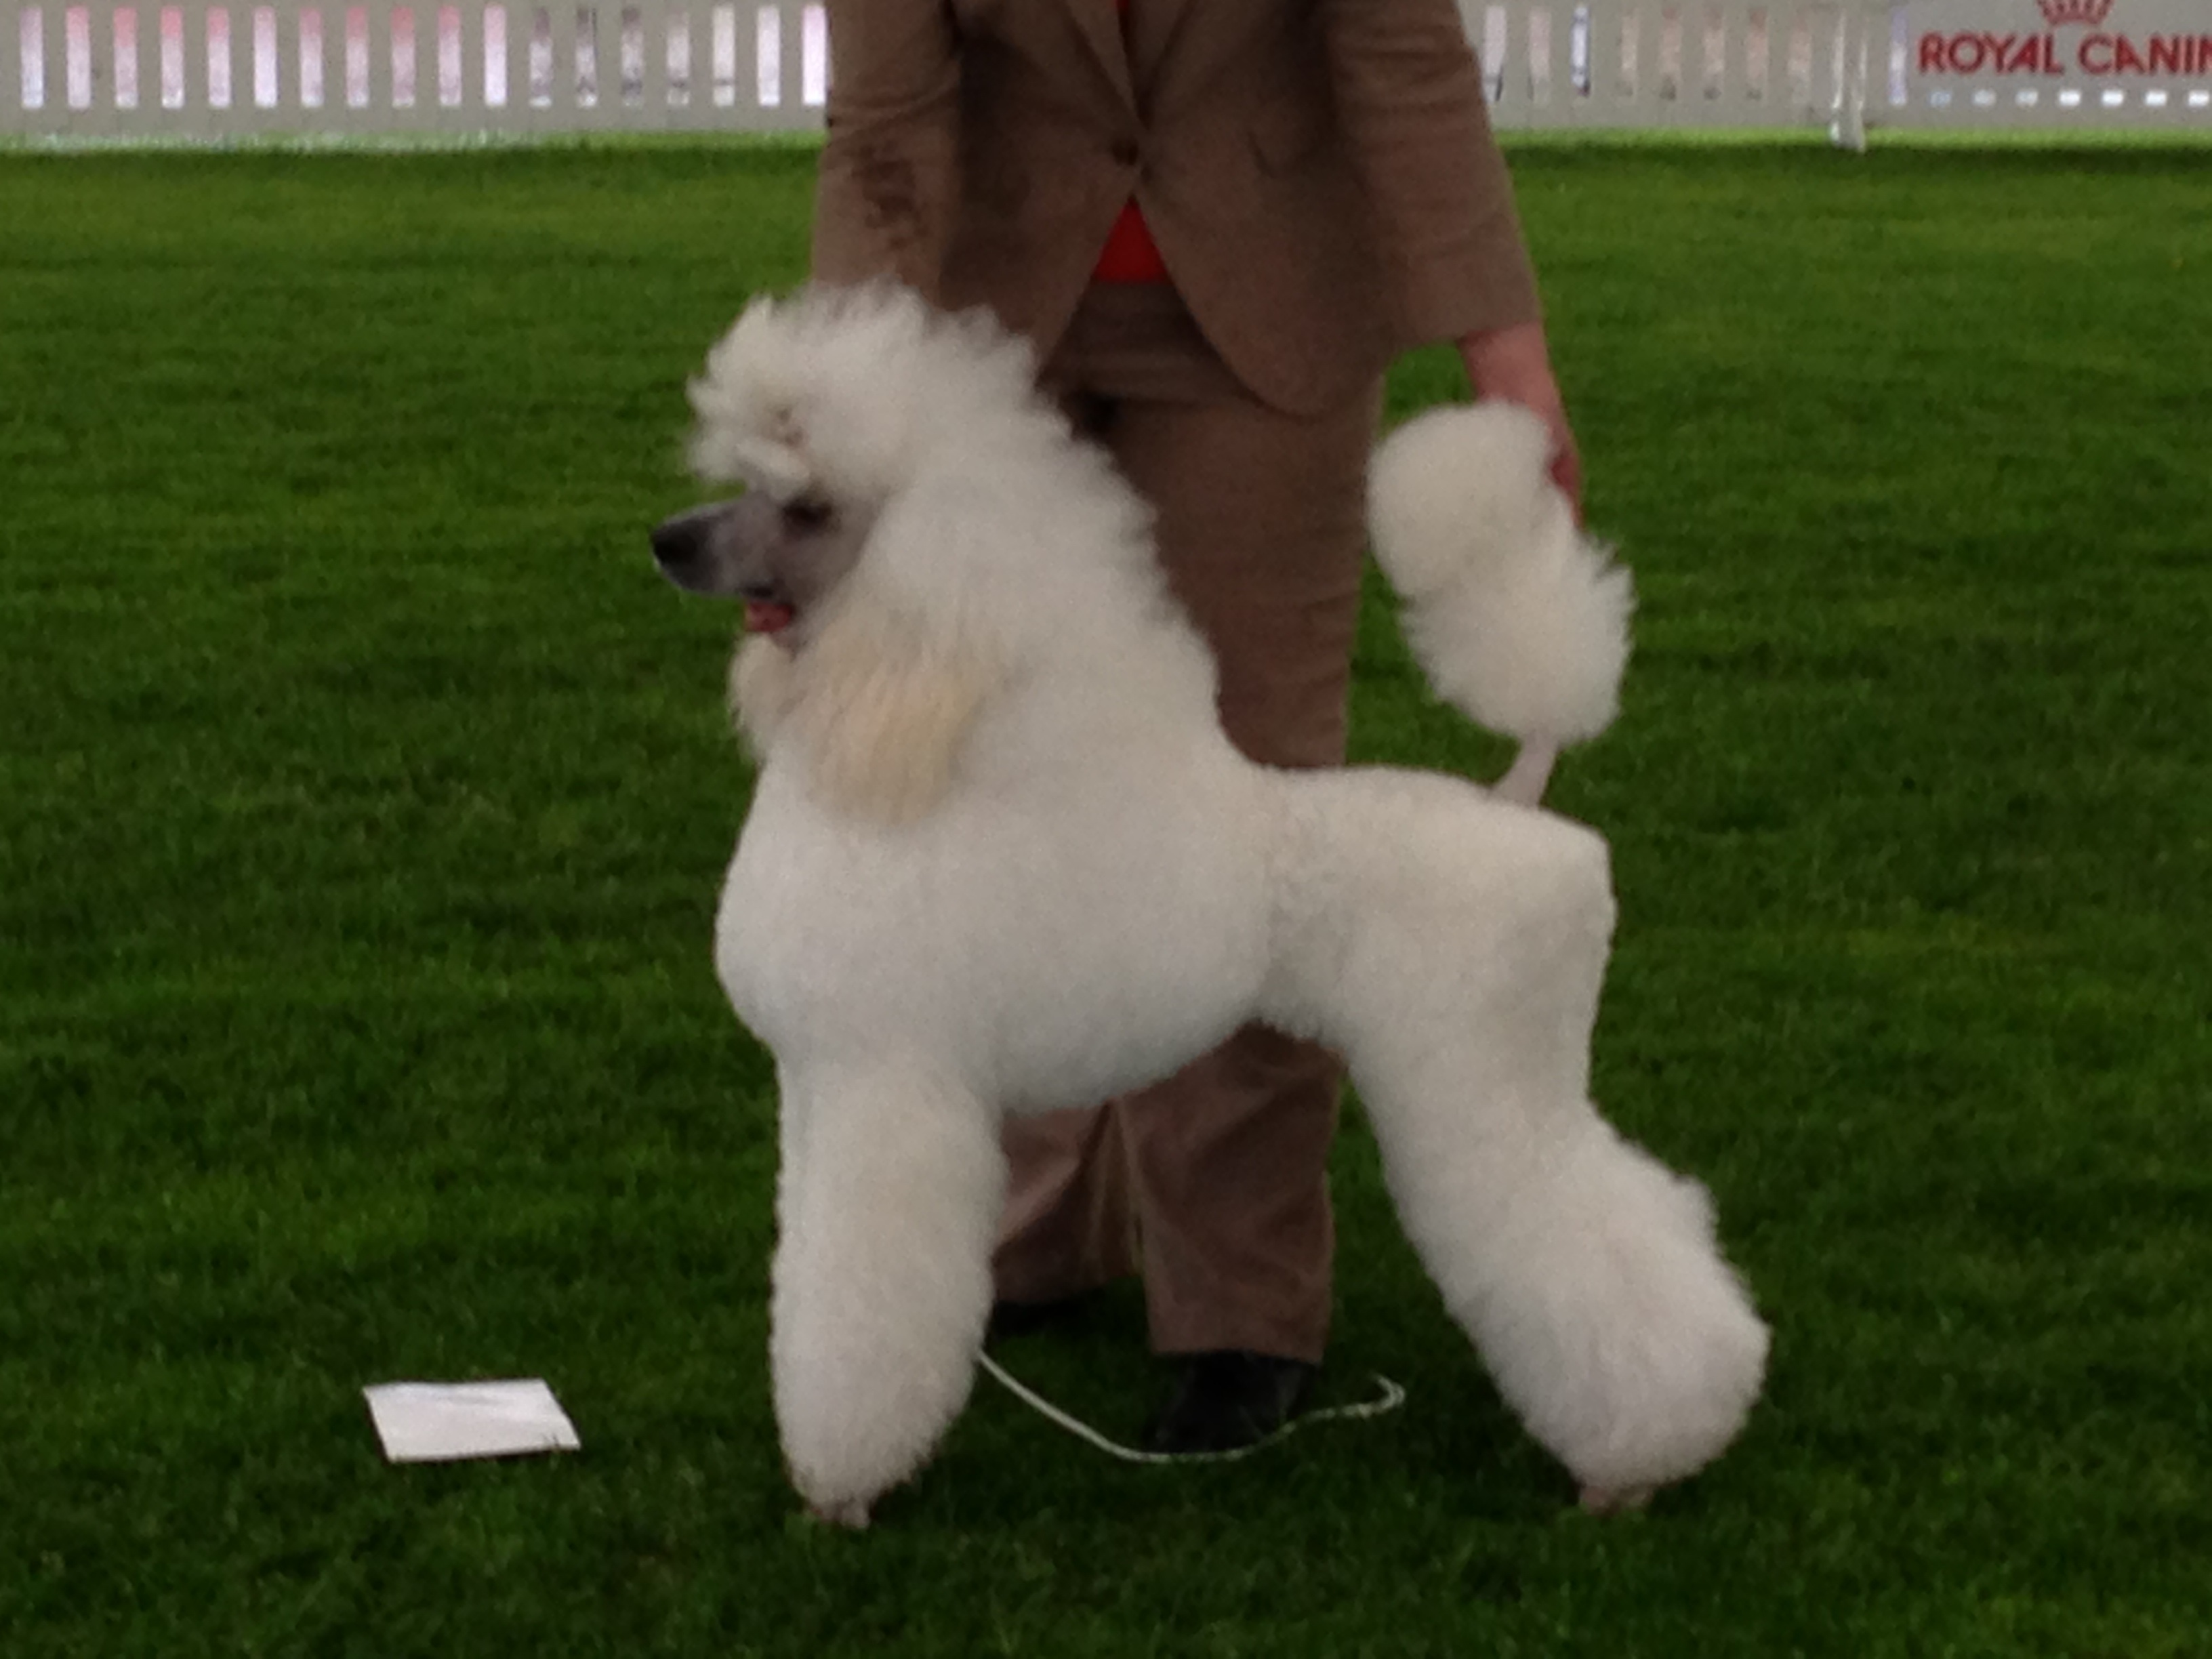
\includegraphics[width=2.0in]{poodle.jpg}
\caption{Poodles with exquisite fur are highly sought after. In fact, some breeders attempt to breed a furrier series. \href{https://commons.wikimedia.org/wiki/File:Poodle,_white_standard_04.jpg}{(Image credit)}}
\end{center}
\end{figure}

The strategy for turnin'-up-the-bass will be as follows \vspace{0.1in}

\begin{center}
  
\includegraphics[width=5in]{fourier_strategy_svg.png}

 \href{https://commons.wikimedia.org/wiki/File:Commutative_diagram_illustrating_problem_solving_via_the_Fourier_transform.svg}{(image credit)}
\end{center}

Once in basis of frequency functions\footnote{I am calling the exponential a `frequency function' because $\exp(i(2\pi fx)) = \cos (2 \pi f x) + i \sin (2 \pi f x)$}, I can just amplify the low-frequency coefficients $$c'_\xi = \begin{cases}
c_\xi & \textrm{if }\xi\textrm{ is a lame treble frequency} \\ 
A(\xi)c_\xi & \textrm{if }\xi\textrm{ is an awesome bass frequency} \\ 
\end{cases} $$

Then I need to convert out of frequency-function basis back to the normal basis. That is what the Inverse Fourier Transform is for.

\subsection{Contravariance}

Note that if we change to $d$-basis, any position-vector before the change must point to the same spot after the change. In order for this to happen, the coordinates have to change in the \textit{opposite} way as the basis changes. For example: if I made the basis vectors twice as big $\vecl{2, 0, 0}\!, \vecl{0, 2, 0}\!, \vecl{0, 0, 2}$, then every vectors coordinates in this basis have to get twice as small in order to point to the same spot. In our equation, $\vec{x}_{(d)} = D^{-1} \vec{x}$, the $d$-components of $\vec{x}$ are proportional $D$-\textbf{inverse}. The coordinates are contravariant with the bases.

In physics, displacement is a vector because it behaves this way. If I change to a different inertial frame of reference (equivalent to a change-of-basis), the coordinates change in the opposite direction and the physical quantity remains unchanged.

This is not true of the triplet containing temperature, charge, and mass. If I change to a different inertial frame, the coordinates of that triplet remain unchanged. That triplet does not constitute not a vector; it is simply three scalars. On the hand, velocity in the $x$-direction, even when considered by itself, is not a scalar. If I change my frame of reference, the velocity in the $x$-direction could change; Instead, we say velocity in the $x$-direction is one component of a vector.

In classical physics, time is a scalar. It is unaffected by changes in frame of reference. But as we shall see later, in relativistic mechanics, time is not a scalar; it is part of a vector.

% \section{Covectors}

% Linear maps $f(\vec{x} + \vec{w}) = f(\vec{x}) + f(\vec{w})$ and $f(a \vec{x}) = a f(\vec{x})$

% Dual space, $V^*$, is a vector space.

% $(f + g)(\vec{x}) = f(\vec{x}) + g(\vec{x})$ and $(af)(\vec{x}) = a (f(\vec{x}))$.

% Derive covector basis.

% Do example.

% If regular vectors are column-vectors, then covectors are row-vectors because $\vec{f}^T \vec{x}$. But this is identical to a inner-product $\langle f, x \rangle$, where $f$ and $x$ are both vectors. (also called $\langle f | x \rangle$ or $[f | x]$, see Bra-ket notation)

% As such, we can think of a covector as $\langle f , \cdot \rangle$.

% % https://en.wikipedia.org/wiki/Dual_space#Finite-dimensional_case

% \section{Transformations of tensors}

% Tensors are defined by how they transform.

% Not all scalars are tensors of rank-(0, 0), but all tensors of rank-(0, 0) are scalars. Temperature is a tensor of rank zero because $T' = T$. Frequency of light is not a tensor of rank-(0, 0).

% While the vector itself is coordinate independent, its individual components are not.

% \section{Einstein notation}

% \subsection{Rules}

% Conventions for naming things.

% % https://en.wikipedia.org/wiki/Einstein_notation#Introduction

% \subsection{Examples}

% % https://en.wikipedia.org/wiki/Einstein_notation#Common_operations_in_this_notation
% % https://en.wikipedia.org/wiki/Ricci_calculus#Notable_tensors

% \subsection{Groups of subscripts}

% % https://en.wikipedia.org/wiki/Ricci_calculus#Upper_and_lower_indices
% % https://en.wikipedia.org/wiki/Ricci_calculus#Symmetric_and_antisymmetric_parts

% % https://en.wikipedia.org/wiki/Penrose_graphical_notation

% \section{Operations on Tensors}

% Tensor products

% Contractions

% Raising/lowering index

% \subsection{Application in rotations}

% \subsection{Application in special relativity}

% Two conventions for the metric tensor

% \section{4 > 3 (more four-vectors)}

% \subsection{Application in electromagnetism}

\end{document}

%%% Local Variables:
%%% mode: latex
%%% TeX-master: t
%%% End:
